\documentclass[xcolor]{beamer}

\usepackage[T1]{fontenc}

\usetheme{Malmoe}
\useoutertheme{infolines}
\useinnertheme{circles}

\makeatletter
\setbeamertemplate{mini frames}{}
\setbeamertemplate{headline}{%
	\begin{beamercolorbox}[ht=2.5ex,dp=1.125ex]{section in head/foot}
		\insertnavigation{\paperwidth}
	\end{beamercolorbox}%
}%
\makeatother
\setbeamertemplate{caption}[numbered]

% Colours defined here
\definecolor{DarkGreen}{HTML}{41964b}
\definecolor{LightGreen}{HTML}{46c755}
\definecolor{FG}{HTML}{ebebeb}
\definecolor{BG2}{HTML}{233628}
\definecolor{BG}{HTML}{202622}

\setbeamercolor{palette primary}{bg=BG, fg=FG}
\setbeamercolor{palette secondary}{bg=BG, fg=FG}
\setbeamercolor{palette tertiary}{bg=BG, fg=FG}
\setbeamercolor{palette quaternary}{bg=BG, fg=FG}

\setbeamercolor{section in head/foot}{bg=BG2, fg=DarkGreen}
\setbeamercolor{subsection in head/foot}{bg=BG2, fg=LightGreen}
\setbeamercolor{page number in head/foot}{bg=BG2, fg=LightGreen}
\setbeamercolor{author in head/foot}{bg=BG2, fg=DarkGreen}
\setbeamercolor{date in head/foot}{bg=BG2, fg=DarkGreen}
\setbeamercolor{title in head/foot}{bg=BG2, fg=LightGreen}

\setbeamercolor{normal text}{fg=FG, bg=BG}
\setbeamercolor{structure}{fg=LightGreen, bg=BG}

\setbeamerfont{subsection in toc}{size=\scriptsize}
\setbeamerfont{section in toc}{size=\footnotesize}

\usefonttheme{serif}

\usepackage{unicode-math}
\setmainfont{Gentium Basic} % Main font
\setmonofont{Fantasque Sans Mono} % Code font

\usepackage{amsmath}
\usepackage{amssymb}
\usepackage{microtype}

\usepackage{listings}
\lstset{%
	language=C,
	frame=single,
	backgroundcolor=\color{BG2},
	basicstyle={\tiny\ttfamily\color{FG}},
	keywordstyle=\color{LightGreen}
}

\usepackage{graphicx}
\graphicspath{{./files/}}

\usepackage{tikz}
\usetikzlibrary{shapes.geometric, positioning}
% tikz style
\tikzstyle{startstop} = [rectangle, rounded corners, minimum width=2cm, minimum height=1cm,text centered, draw=white]
\tikzstyle{io} = [trapezium, trapezium left angle=70, trapezium right angle=110, minimum width=2cm, minimum height=0.75cm, text centered, draw=white]
\tikzstyle{process} = [rectangle, minimum width=2cm, minimum height=1cm, text centered, draw=white]
\tikzstyle{decision} = [diamond, minimum width=2cm, minimum height=1cm, text centered, draw=white]

\usepackage{cancel}

\author[Kyu-Sang Kim]{Kyu-Sang Kim\\z5208931\\\vspace{0.2cm}Supervised by Andrew Taylor (UNSW)\\Assessed by John Shepherd (UNSW)}
\title[Thesis B Seminar]{A Testing Tool for Introductory Programming Courses}
\subtitle{Thesis B Seminar}
\date{Term 2, 2022}

\begin{document}

\begin{frame}
	\titlepage
\end{frame}

\AtBeginSection[]{
	\begin{frame}
		\frametitle{Contents}

		\centering
		\begin{columns}
			\begin{column}{0.75\textwidth}
				\tableofcontents[currentsection]
			\end{column}
			\begin{column}{0.15\textwidth}
				% Use this for anything you want to display alongside the contents
			\end{column}
		\end{columns}
	\end{frame}
}

\section{Introduction}
\subsection{Thesis Statement}
\begin{frame}
	\frametitle{Thesis Statement}
	\textbf{A user-friendly and maintainable general code testing tool is important to streamline the administration of introductory programming courses}
	\\~\\
	\pause
	We will:
	\begin{enumerate}
		\item Develop an extensible and easy to use software package which parses and runs pre-written tests on submitted code
		\pause
		\item Implement development procedures that minimise both current and future technical debt
		\pause
		\item Remediate known flaws in the existing autotest package
		\pause
		\item Maintain backwards compatibility with legacy tests written for the existing autotest package
		\pause
		\item Perform proving and performance tests on the new software package
		\pause
		\item Deprecate and replace the existing autotest used for introductory programming courses at UNSW CSE
	\end{enumerate}
\end{frame}

\subsection{Plan}
\begin{frame}
	\frametitle{Schedule}
	The original plan was set to the following:
	\begin{enumerate}
	\item Thesis B:
	\begin{itemize}
		\item Implement Core Main Module
		\pause
		\item Implement Core Testcase Parser Module
		\pause
		\item Implement Core Testcase Runner Module
		\pause
		\item Run correctness and performance testing on Parser and Runner
		\pause
	\end{itemize}
	\item Thesis C:
	\begin{itemize}
		\item Implement Core Testcase Program Correctness Module
		\pause
		\item Implement any extensions that have been deemed necessary
		\pause
		\item Run correctness and performance testing on complete package and make final adjustments
		\pause
	\end{itemize}
	\end{enumerate}
	This presentation will discuss work done for Thesis B. 
\end{frame}

\section{Thesis B Work}
\subsection{Overview}
\begin{frame}
	\frametitle{Summary}
	The majority of thesis B was on enabling development.\\
	This involved:
	\begin{itemize}
		\item Designing the core architecture
		\pause
		\item Porting over legacy code to modules for the new architecture
		\pause
		\item Designing and implementing the new Test definition
		\pause
		\item Designing and implementing the new Thesis B modules
		\pause
		\item Running performance and correctness tests on legacy, ported and new versions of the same modules
		\pause
		\item Setting up an automated testing and styling infrastructure
	\end{itemize}
\end{frame}

\subsection{Core Architecture}
\begin{frame}
	\frametitle{Modular Design}
	\begin{itemize}
		\item A modular design has been selected for the new autotest
		\pause
		\item Modules are an established design pattern that fits the purpose of autotest
		\pause
		\item Enables components of high complexity to be rendered mostly if not completely separate from the internal implementations of other components
		\pause
		\item Each component will be inclined to do only \textbf{\underline{one}} task well
		\pause
		\item Enables easier swapping of components with minimal to no code changes other than import statements
		\pause
		\item Maintenance and Improvements can be tested without an overhaul
		\pause
		\item Abstract Class design allows for easier novel design and implementation of pre-existing modules
	\end{itemize}
\end{frame}

\begin{frame}
	\frametitle{Architecture Diagram}
	\begin{figure}
		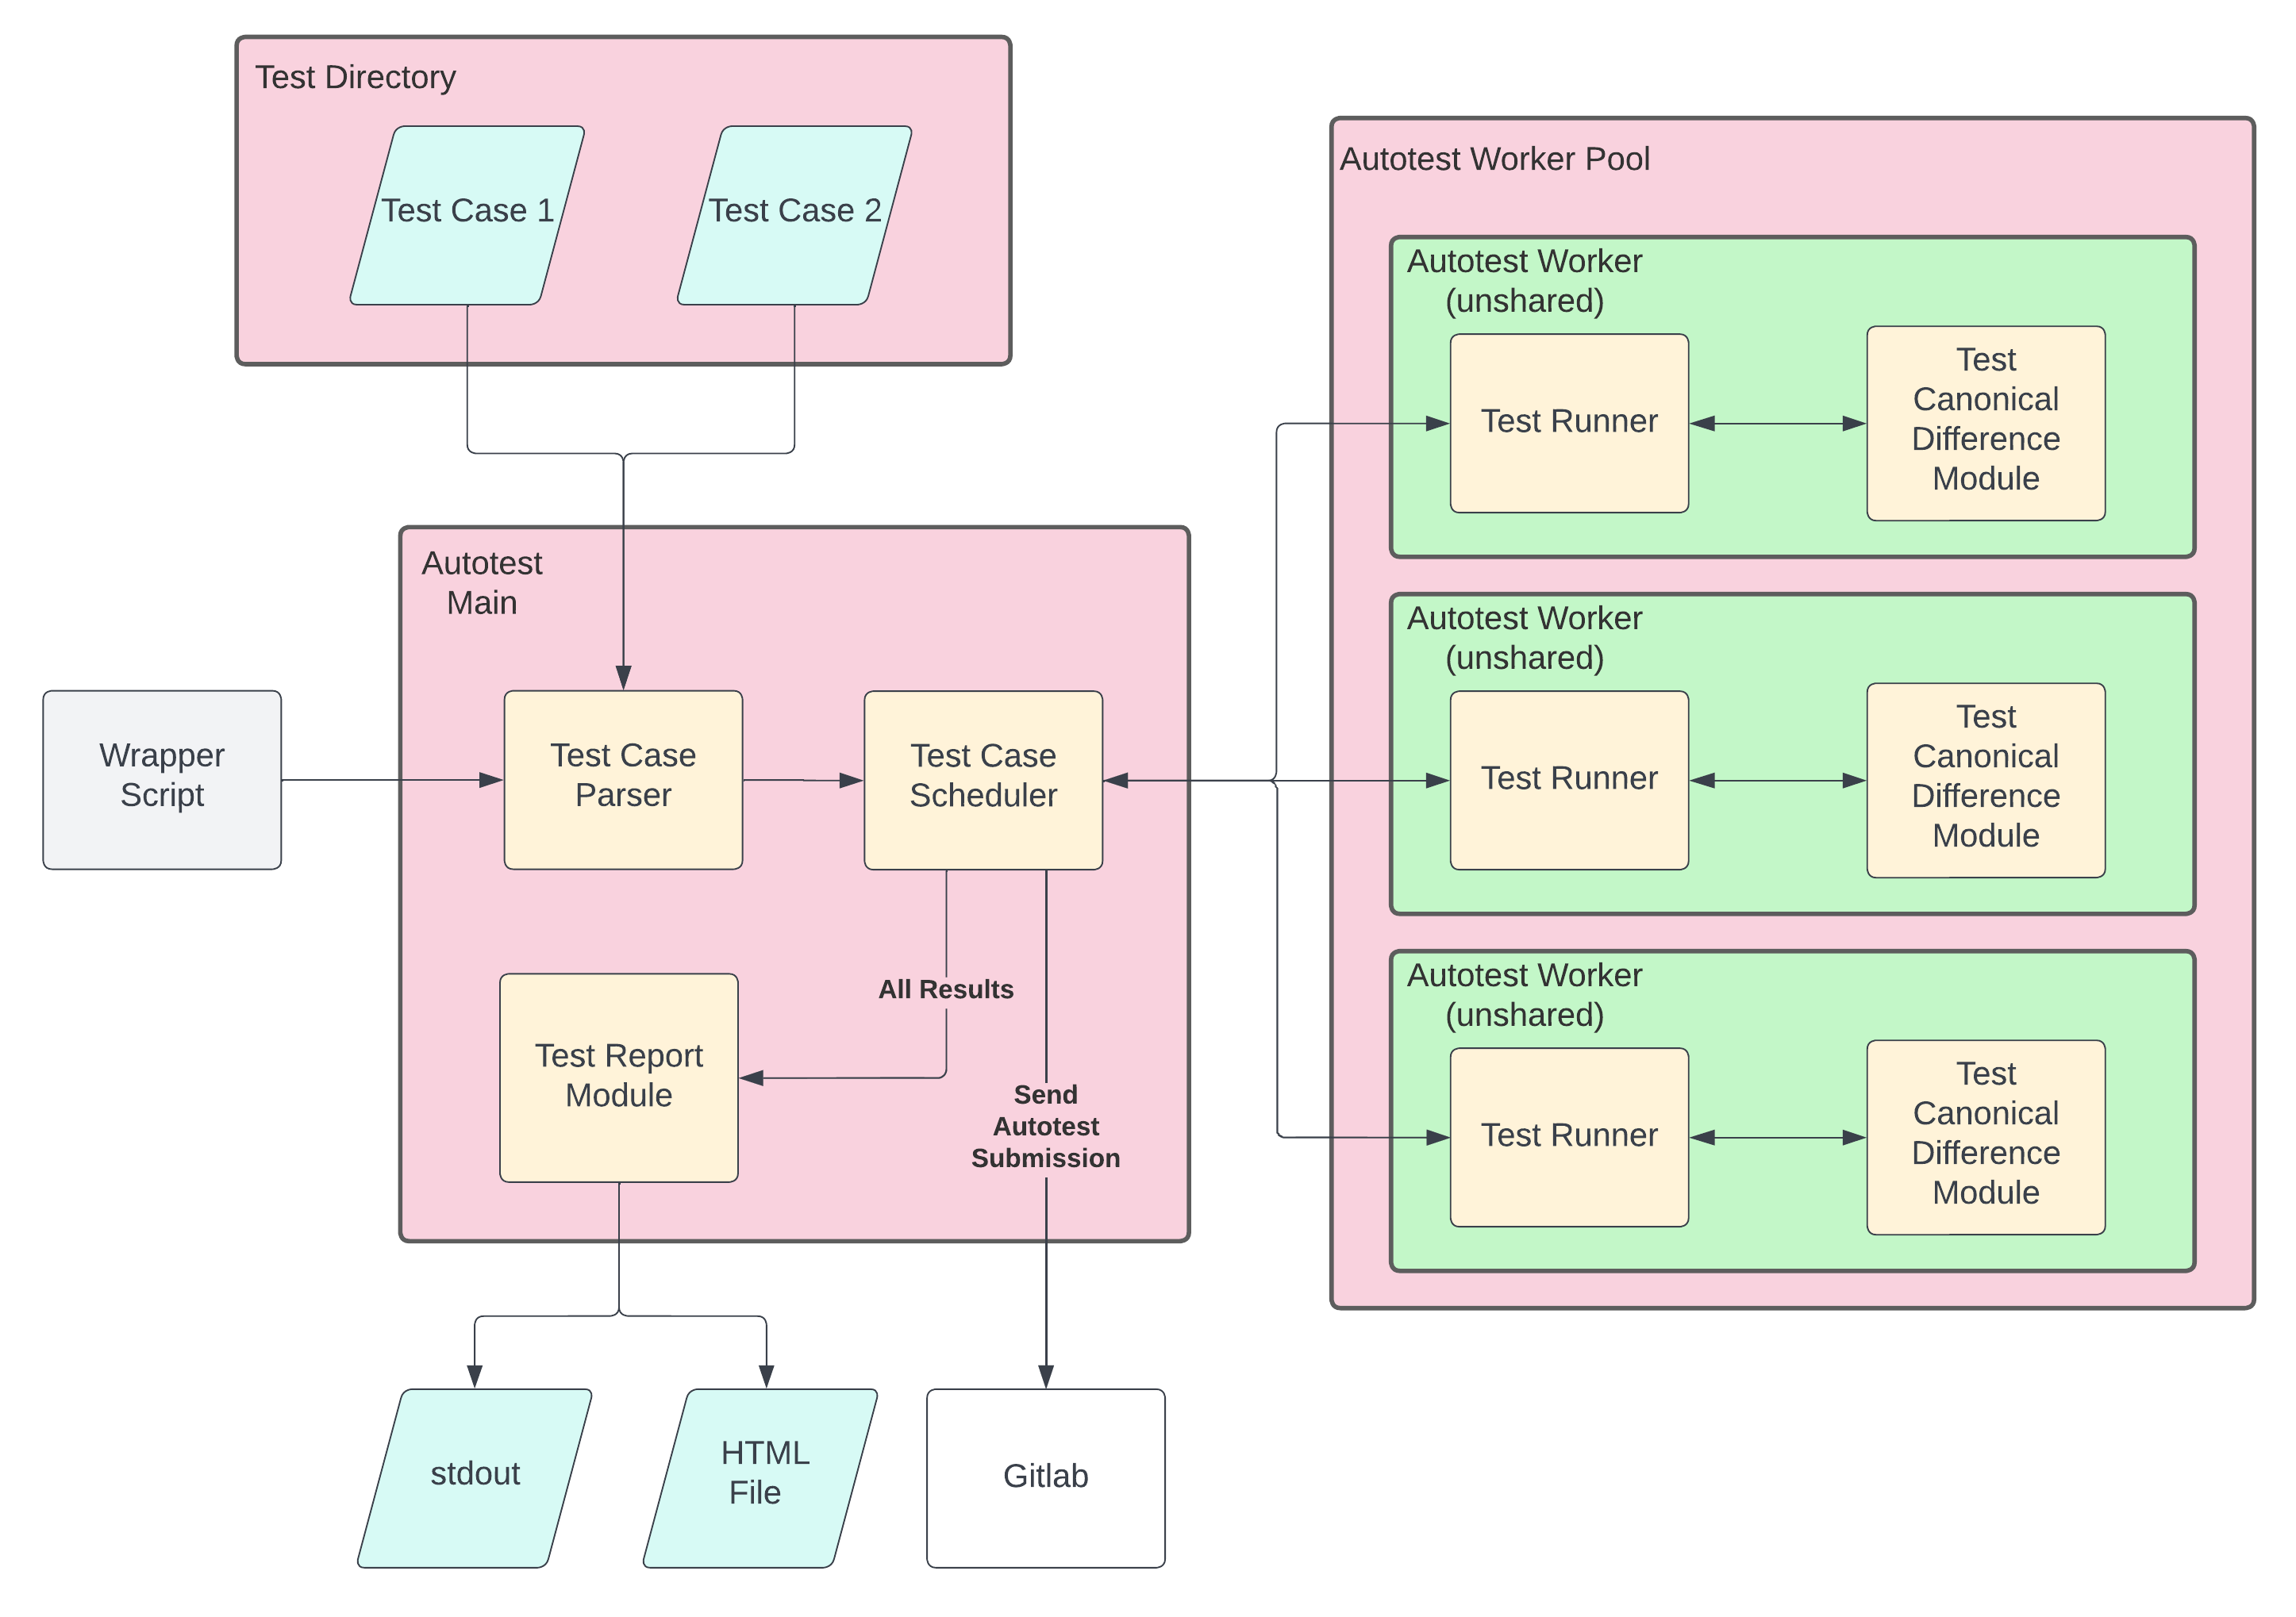
\includegraphics[width=\textwidth, height=0.85\textheight, keepaspectratio=true]{architecture}
	\end{figure}
\end{frame}

\subsection{Modules}
\begin{frame}
	\frametitle{Core Module}
	\textbf{Purpose:} The ``Main" Program\\
	\begin{itemize}
		\item Coordinates execution of modules
		\pause
		\item Facilitates information transfer between modules
		\pause
		\item Exposed only to the abstraction of each module
		\pause
		\item Direct code only for optional ``administrative" tasks
	\end{itemize}
\end{frame}

\begin{frame}
	\frametitle{Parser Module}
	\textbf{Purpose:} Argument and Test Case Parser\\
	\begin{itemize}
		\item Ingests autotest parameters for processing into usable information
		\pause
		\item Retrieves relevant autotest test cases and processes them into test definitions
		\pause
		\item Minimised exposure to test definition
		\pause
		\item Most complex component in the entire package
		\pause
	\end{itemize}
	\textbf{Changes:}
	\begin{itemize}
		\item Legacy parser code carries too much technical debt for a refactor (circular dependency hell etc.)
		\pause
		\item Writing a new one is unrealistic due to possible correctness concerns
		\pause
		\item \textbf{Scope Change - Salvaged/Ported legacy + adaptor}
		\pause
	\end{itemize}
	\textbf{Status: Completed}
\end{frame}

\begin{frame}
	\frametitle{Test Case Definition}
	\textbf{Purpose:} Defines a test and the information contained within it\\
	\begin{itemize}
		\item Used by the parser to generate the test definitions to be scheduled and executed
		\pause
		\item Contains all information involving each test such as required files, pre-checks etc.
		\pause
		\item Easily expanded for new features per design
		\pause
	\end{itemize}
	\textbf{Status: Semi-Completed - Awaiting Possible Modifications}
\end{frame}

\begin{frame}
	\frametitle{Test Case Scheduler Module}
	\textbf{Purpose:} Test runner pool manager and test allocator\\
	\begin{itemize}
		\item Ingests parameters to initialise a container pool that enables concurrent execution of tests
		\pause
		\item Schedules ingested test definitions to free workers in container pool via producer-consumer pattern with synchronisation primitives
		\pause
		\item Manages worker instances and cleanup on completion/process signal
		\pause
		\item Expected to deliver the most performance benefit compared to legacy by eliminating Single Instruction, Single Data (SISD) limitation (AKA single-thread, single-process)
		\pause
	\end{itemize}
	\textbf{Status: In Progress}
\end{frame}

\begin{frame}
	\frametitle{Test Case Runner Module}
	\textbf{Purpose:} Container management and test runner\\
	\begin{itemize}
		\item Initialises a worker which accepts test definitions until no more can be found or signal sent
		\pause
		\item Utilises \textit{unshare} to implement containerised execution of given test
		\pause
		\item Manages container environment setup and cleanup for each test
		\pause
		\item Expected to deliver on security needs
		\pause
	\end{itemize}
	\textbf{Changes:}
	\begin{itemize}
		\item \textbf{Scope Change - Compartmentalisation is now included in scope}
		\pause
	\end{itemize}
	\textbf{Status: In Progress}
\end{frame}

\begin{frame}
	\frametitle{Why \textit{unshare}?}
	\textbf{Purpose:} \textit{unshare} is a Linux kernel system call introduced in 2008 that allows a process to \textit{disassociate} some components of it's inherited process context
	\pause
	\\~\\
	In the case of autotest, \textit{unshare} allows processes to \textit{disassociate} a \textit{user namespace} and replace it with a subordinate that cannot "see`` the original
	\pause
	\\~\\
	The same can also be done for network access, file system mounts etc.
\end{frame}

\begin{frame}
	\frametitle{Why \textit{unshare}?}
	\textbf{What does \textit{unshare} solve?}
	\pause
	\begin{itemize}
		\item Many courses run autotest with their class account (cs1521) when marking which has led to concerns of malicious programs inheriting an overly privileged user id
		\pause
		\item With \textit{unshare}, a very lightweight fakeroot container can be created for an \textbf{autotest worker} to execute tests to eliminate most risks of damage on the host file system \textbf{\underline{without needing root access (rootless)}}
	\end{itemize}
	\pause
	\textbf{Why not alternatives?}\\
	\pause
	\begin{itemize}
		\item Most of the Linux container engines available (\textbf{Docker}, \textbf{Bubblewrap} etc.) have too much overhead and are far too powerful for the job
		\pause
		\item Although rootless versions of some engines exist, it is considered to be ``inferior" and task-specific support/documentation has been minimal
		\pause
		\item Most engines wrap around \textit{unshare} to deliver capabilities
	\end{itemize}
\end{frame}

\begin{frame}
	\frametitle{Test Case Canonical Difference Module}
	\textbf{Purpose:} Test correctness checker and test case report generation\\
	\begin{itemize}
		\item Compares output of executed test to expected output
		\pause
		\item Reports success when output matches expected
		\pause
		\item Reports failure when out does not match expected with a report on differences and test reproduction information
		\pause
		\item Should report similar if not better information than what legacy currently provides
		\pause
	\end{itemize}
	\textbf{Status: Planned}
\end{frame}

\begin{frame}
	\frametitle{Test Case Report Module}
	\textbf{Purpose:} Optional HTML report generation\\
	\begin{itemize}
		\item Converts autotest output to more readable HTML form
		\pause
		\item Assists in course administration with forums by making output much more easier to copy by students
		\pause
	\end{itemize}
	\textbf{Status: Planned as extension - could be dropped}
\end{frame}

\subsection{Demo \& What was supposed to happen}
\begin{frame}
	\frametitle{Demo}
	\begin{itemize}
		\item Main module is regulating how the parser and test case scheduler modules interact
		\item Legacy Parser has been cut down, revamped and ported over to the new architecture
		\item Observe that tests are being parsed correctly and from the correct directory
	\end{itemize}
\end{frame}

\begin{frame}
	\frametitle{What was supposed to happen}
	If we had implemented all of Thesis B as originally planned:
	\begin{itemize}
		\item Main module initialises the test scheduler with parsed parameters
		\pause
		\item Test scheduler spins up a parameterised number of autotest workers
		\pause
		\item Each autotest worker will create an execution environment with \textit{unshare} and await tests
		\pause
		\item Main module queues tests in an array to be consumed by free workers
		\pause
		\item Autotest worker consumes test by setting up any pre-test requirements, executing the test in \textit{unshare} environment, cleaning up and populating test instance with produced output
		\pause
		\item Autotest worker sends back populated test back to Main module
		\pause
		\item Main module makes basic output comparison to determine if test has passed or failed before printing result to stdout
	\end{itemize}
\end{frame}

\section{Thesis C}
\subsection{Thesis B Post-Mortem}
\begin{frame}
	\frametitle{What went wrong?}
	\begin{itemize}
		\item Initial goal to refactor the test parser was more challenging than originally anticipated
		\pause
		\item Too much time was spent on the parser before scope was revised
		\pause
		\item My own expectations on the time I thought I had available for Thesis B were not met
	\end{itemize}
\end{frame}

\begin{frame}
	\frametitle{What will be done?}
	\begin{itemize}
		\item Scope Revisions
		\pause
		\item Higher allocation of weekly time to Thesis C
	\end{itemize}
\end{frame}

\subsection{Thesis C Revised Scope}
\begin{frame}
	\frametitle{Scope Revision}
	To make thesis C more realistic with the remaining time, the following changes have been made:
	\begin{itemize}
		\item Removal of the following clause from the thesis statement:
		\begin{itemize}
			\item Deprecate and replace the existing autotest used for introductory programming courses at UNSW CSE
		\end{itemize}
		\pause
		\item Refactoring of the legacy parser is to be considered ``out of scope" for this thesis
	\end{itemize}
	
\end{frame}

\subsection{Thesis C Plan}
\begin{frame}
	\frametitle{Thesis C Plan}
	\begin{itemize}
		\item Implement remaining work for Test Definition, Test Scheduler and Autotest Worker
		\pause
		\item Finalise location and concrete implementation of Canonical Difference module
		\pause
		\item Assess whether making the optional Report module will be viable within the remaining time
		\pause
		\item Perform correctness and performance testing for the final report
		\pause
		\item Finalise Thesis C demo plan and slides
		\pause
		\item Finalise and submit Thesis C report
		\pause
	\end{itemize}
	\textit{\textbf{Thank you for attending!} Questions?}
\end{frame}


\end{document}
